\documentclass[../main.tex]{subfiles}
\graphicspath{{\subfix{../Images/}}}

\begin{document}

\chapter{Appendix B. The Cg Runtime}

\section{B.1 What Is the Cg Runtime?}

Cg programs supply programs for GPUs, but they need the support of an application to render images. To interface Cg programs with an application, you must do two things:

\begin{enumerate}
\item \textbf{Compile the programs for the appropriate profile.} This step translates your Cg program into a form that is compatible with the 3D programming interface used by the application and the underlying hardware.
\item \textbf{Link the programs to the application program.} This step allows the application to configure the program for execution, and to feed it varying and uniform parameters.
\end{enumerate}

You can choose when you want to perform these operations. You can perform them at \textit{compile time}, when the application program is compiled into an executable, or you can perform them at \textit{runtime}, when the application is actually executed. The Cg runtime is a set of application programming interfaces (APIs) that allows an application to compile and link Cg programs at runtime.

\section{B.2 Why Use the Cg Runtime?}

\subsection{B.2.1 Future-Proofing}

Most applications need to run on a variety of GPUs with various levels of functionality, so these applications need to run on a variety of profiles. If an application precompiles its Cg programs (at compile time), it must store a precompiled version of each program for each profile. Although possible, the precompiled approach is cumbersome for an application that uses many Cg programs. What's worse, the Cg programs become frozen in time. By precompiling Cg programs, an application sacrifices the optimizations that future compilers could offer.

In contrast, Cg programs compiled by applications at runtime benefit from future compiler optimizations for existing profiles. And these programs can run on future profiles corresponding to new hardware and 3D API functionality that did not exist when the application's Cg programs were written.

\subsection{B.2.2 No Dependency Issues}

If you link a compiled Cg program to an application, the application becomes tied to the result of the compilation, particularly with respect to how the compiler allocates parameters. The application program would have to refer to the Cg program input parameters by using the hardware register names that the Cg compiler outputs. This approach causes two significant problems:

\begin{enumerate}
\item Register names cannot be easily matched to the corresponding meaningful names in the Cg program without looking at the compiler output.
\item Register allocations can change each time the Cg program, the Cg compiler, or the compilation profile changes. This means you would have to update the application each time as well, which would be inconvenient.
\end{enumerate}

In contrast, linking a Cg program to the application program at runtime removes the dependency on the Cg compiler. With the Cg runtime, you only need to alter the application code when you add, delete, or rename Cg input parameters.

\subsection{B.2.3 Input Parameter Management}

The Cg runtime also offers facilities to manage the input parameters of the Cg program. In particular, it makes data types such as arrays and matrices easier to deal with.

These additional functions also encompass the necessary 3D API calls to minimize code length and reduce programmer errors.

\section{B.3 How Does the Cg Runtime Work?}

Figure \ref{fig:B-1} shows the three libraries that make up the Cg runtime API.

\begin{figure}
    \centering
    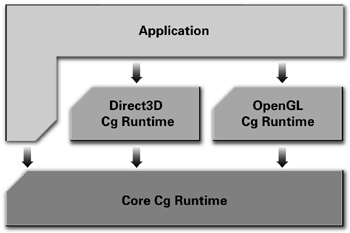
\includegraphics[width=0.75\linewidth]{figb_1.jpg}
    \caption{Figure B-1 The Parts of the Cg Runtime API}
    \label{fig:B-1}
\end{figure}

\begin{itemize}
\item A core set of functions and structures encapsulating the 3D API–independent functionality of the runtime.
\item An OpenGL-specific set of functions built on top of the core set.
\item A Direct3D-specific set of functions built on top of the core set.
\end{itemize}

To make it easier for application writers, the OpenGL and Direct3D libraries each adopt the philosophy and data structure style of their respective APIs. You need only link with the 3D API–specific Cg runtime library for the 3D API your application uses. Therefore, most applications use either the OpenGL or Direct3D Cg runtime library.

The rest of this appendix provides code fragments, written in C, for using the Cg runtime in the framework of an application. Each step includes source code for OpenGL and Direct3D programming.

Functions that involve only pure Cg resource management belong to the core runtime and have a \textbf{cg} prefix. In these cases, the same code is used for OpenGL and Direct3D.

When functions from the OpenGL or Direct3D Cg runtime libraries are used, notice that the API name is indicated by the function name. Functions belonging to the OpenGL Cg runtime library have a \textbf{cgGL} prefix, and functions in the Direct3D Cg runtime library have a \textbf{cgD3D8} or \textbf{cgD3D9} prefix, for DirectX 8 and DirectX 9, respectively. In the examples that follow, we show the DirectX 9 versions of the examples. Replacing "\textbf{D3D9}" with "\textbf{D3D8}" will produce the DirectX 8 versions of the same examples. Note that the functions we list here take the same parameters in DirectX 8 and DirectX 9. In general, this is not always the case.

\subsection{B.3.1 Header Files}

Here's how to include the core Cg runtime API into your C or C++ program:

\FloatBarrier
\begin{lstlisting}
#include <Cg/cg.h>
\end{lstlisting}
\FloatBarrier

Here's how to include the OpenGL-specific Cg runtime API:

\FloatBarrier
\begin{lstlisting}
#include <Cg/cgGL.h>
\end{lstlisting}
\FloatBarrier

Here's how to include the DirectX 8–specific Cg runtime API:

\FloatBarrier
\begin{lstlisting}
#include <Cg/cgD3D8.h>
\end{lstlisting}
\FloatBarrier

Here's how to include the DirectX 9–specific Cg runtime API:

\FloatBarrier
\begin{lstlisting}
#include <Cg/cgD3D9.h>
\end{lstlisting}
\FloatBarrier

\subsection{B.3.2 Creating a Context}

A context is a container for Cg programs. It holds the Cg programs you load, as well as their shared data.

Here's how to create a context:

\FloatBarrier
\begin{lstlisting}
CGcontext context = cgCreateContext();
\end{lstlisting}
\FloatBarrier

\subsection{B.3.3 Compiling a Program}

Compile a Cg program by adding it to a context, using the \textbf{cgCreateProgram} function:

\FloatBarrier
\begin{lstlisting}
CGprogram program =
cgCreateProgram(context,             // from cgCreateContext
                CG_SOURCE,           // type: source or object
                programString,       // program text/data
                profile,             // profile
                "main",              // entry function name
                args);               // compiler options
\end{lstlisting}
\FloatBarrier

The \textbf{CG_SOURCE} parameter indicates that the following string argument, \textbf{programString}, is an array of bytes containing Cg source code, not precompiled code. The Cg runtime does let you create a program from compiled code (called object code) by using the \textbf{CG_OBJECT} rather than \textbf{CG_SOURCE} parameter, if you want to.

\textbf{profile} specifies the profile for which the program will be compiled—for example, \textbf{CG_PROFILE_ARBVP1} for OpenGL applications, or \textbf{CG_PROFILE_VS_2_0} for Direct3D applications. The \textbf{main} string parameter gives the name of the function to use as the entry function for your program. Finally, \textbf{args} is a list of strings that supplies options to the compiler.

\subsection{B.3.4 Loading a Program}

After you compile a program, you need to pass the resulting object code to the 3D API that you are using. For this, you need to invoke the Cg runtime's 3D API–specific functions.

In OpenGL, you load a program like this:

\FloatBarrier
\begin{lstlisting}
cgGLLoadProgram(program);
\end{lstlisting}
\FloatBarrier

The Direct3D-specific functions require the Direct3D device structure in order to make the necessary Direct3D calls. The application passes it to the runtime using the following call:

\FloatBarrier
\begin{lstlisting}
cgD3D9SetDevice(device);
\end{lstlisting}
\FloatBarrier

You must do this every time a new Direct3D device is created, typically only at the beginning of the application.

You can then load a Cg program this way in Direct3D 9:

\FloatBarrier
\begin{lstlisting}
cgD3D9LoadProgram(program,             // CGprogram
                  false,               // Parameter shadowing
                  0);                  // Assembly flags
\end{lstlisting}
\FloatBarrier

or this way in Direct3D 8:

\FloatBarrier
\begin{lstlisting}
cgD3D8LoadProgram(program,             // CGprogram
                  false,               // Parameter shadowing
                  0,                   // Assembly flags
                  0,                   // Vertex shader usage
                  vertexDeclaration);  // Vertex declaration
\end{lstlisting}
\FloatBarrier

\textbf{vertexDeclaration} is the Direct3D vertex declaration array that describes where to find the necessary vertex attributes in the vertex streams.

\subsection{B.3.5 Modifying the Program Parameters}

The runtime lets you modify the values of your program parameters. The first step is to get a handle to the parameter:

\FloatBarrier
\begin{lstlisting}
CGparameter myParameter = cgGetNamedParameter(program,
                                              "myParameter");
\end{lstlisting}
\FloatBarrier

\textbf{myParameter} is the name of the parameter as it appears in the program source code.

The second step is to set the parameter value. The function used depends on the parameter type.

Here is an example in OpenGL:

\FloatBarrier
\begin{lstlisting}
cgGLSetParameter4fv(myParameter, value);
\end{lstlisting}
\FloatBarrier

Here is the same example in Direct3D:

\FloatBarrier
\begin{lstlisting}
cgD3D9SetUniform(myParameter, value);
\end{lstlisting}
\FloatBarrier

These function calls assign the four floating-point values contained in the array \textbf{value} to the parameter \textbf{myParameter} (assumed to be of type \textbf{float4}).

In both APIs, there are variants of these calls to set matrices, arrays, textures, and texture states.

\subsection{B.3.6 Executing a Program}

Before you can execute a program in OpenGL, you must enable its corresponding profile. For example:

\FloatBarrier
\begin{lstlisting}
cgGLEnableProfile(CG_PROFILE_ARBVP1);
\end{lstlisting}
\FloatBarrier

In Direct3D, nothing special needs to be done to enable a specific profile.

Next, you bind the program to the current 3D API state. This means that it will execute, in the subsequent drawing calls, for every vertex (in the case of a vertex program) and for every fragment (in the case of a fragment program).

Here's how to bind a program in OpenGL:

\FloatBarrier
\begin{lstlisting}
cgGLBindProgram(program);
\end{lstlisting}
\FloatBarrier

Here's how to bind a program in Direct3D:

\FloatBarrier
\begin{lstlisting}
cgD3D9BindProgram(program);
\end{lstlisting}
\FloatBarrier

You can bind only one vertex and one fragment program at a time for a particular profile. Therefore, the same vertex program is executed as long as no other vertex program is bound. Similarly, the same fragment program is executed as long as no other fragment program is bound.

In OpenGL, disable profiles with the following call:

\FloatBarrier
\begin{lstlisting}
cgGLDisableProfile(CG_PROFILE_ARBVP1);
\end{lstlisting}
\FloatBarrier

Disabling a profile issues commands, based on the profile, to return OpenGL to its fixed-function mode.

\subsection{B.3.7 Releasing Resources}

If your application no longer needs a Cg program, it is good programming practice to free the resources maintained for the program by the Cg runtime. Because the Direct3D runtime keeps an internal reference to the Direct3D device, you must tell it to release this reference when you finish using the Direct3D runtime. This is done with the following call:

\FloatBarrier
\begin{lstlisting}
cgD3D9SetDevice(0);
\end{lstlisting}
\FloatBarrier

To free resources allocated for a single program, use this function call:

\FloatBarrier
\begin{lstlisting}
cgDestroyProgram(program);
\end{lstlisting}
\FloatBarrier

To free all the resources allocated for a context, use this function call:

\FloatBarrier
\begin{lstlisting}
cgDestroyContext(context);
\end{lstlisting}
\FloatBarrier

Note that destroying a context destroys all the programs it contains as well.

\subsection{B.3.8 Handling Errors}

The core Cg runtime reports an error by setting a global variable that contains the error code. You can query it, as well as the corresponding error string, in the following way:

\FloatBarrier
\begin{lstlisting}
CGerror error = cgGetError();
const char* errorString = cgGetErrorString(error);
\end{lstlisting}
\FloatBarrier

Each time an error occurs, the core library also calls a callback function optionally provided by the application. This callback function would usually call \textbf{cgGetError}:

\FloatBarrier
\begin{lstlisting}
void MyErrorCallback(void)
{
  const char* errorString = cgGetErrorString(cgGetError());
  printf(logfile, "Cg error: %s", errorString);
}

cgSetErrorCallback(MyErrorCallback);
\end{lstlisting}
\FloatBarrier

Calls to 3D API–specific Cg runtime functions can also generate API-specific errors. For the OpenGL Cg runtime library, they are checked using \textbf{glGetError}. Most of the Direct3D Cg runtime library functions also return a Direct3D error code (\textbf{HRESULT}). Similar to the Direct3D runtime, the Direct3D Cg runtime library can be run in a debug mode, provided you use the debug version of the Direct3D Cg DLL. This mode is enabled by the following call:

\FloatBarrier
\begin{lstlisting}
cgD3D9EnableDebugTracing(true);
\end{lstlisting}
\FloatBarrier

In this mode, many helpful messages and traces will be output to the debug output console.

\section{B.4 More Details}

The latest information and documentation about the Cg runtime is available at the NVIDIA Cg Web site:

\textbf{http://developer.nvidia.com/Cg}

\end{document}